\documentclass[
size=17pt,
paper=smartboard,
mode=present,
display=slidesnotes,
style=paintings,
nopagebreaks,
blackslide,
fleqn]{powerdot}

% styles: sailor, paintings
% wj capsules prettybox
% mode = handout or present


\newcommand{\palette}{Moitessier}
% palettes:
%    - sailor: Sea, River, Wine, Chocolate, Cocktail 
%    - paintings: Syndics, Skater, GoldenGate, Moitessier, PearlEarring, Lamentation, HolyWood, Europa, MayThird, Charon 

\newcommand{\cursopequeno}{EC01045 PDS}
\newcommand{\cursogrande}{\Large EC01045 -- Processamento digital de sinais}

\usepackage{amsmath,graphicx,color,amsfonts}
\usepackage[brazilian]{babel}
\usepackage[utf8]{inputenc}
\usepackage{bbding}

\author{Ronaldo de Freitas Zampolo\\FCT-ITEC-UFPA}
\date{ERE 2020}


\pdsetup{
   lf = {\cursopequeno},
   rf = {Sinais e Sistemas Discretos},
   palette = \palette,randomdots={false},
   cf={\theslide}
}

\title{\cursogrande\\ \vspace{1cm}Sinais e sistemas discretos}

\begin{document}

   \maketitle[randomdots={false}]
   \begin{slide}{Agenda}
      \tableofcontents[content=sections]
   \end{slide}

\section[slide=true]{Sinais discretos: representação e amostragem}
   \begin{slide}[toc=]{Representação e amostragem}
      \begin{itemize}
         \item Representação:
         \begin{itemize}
            \item Sequência de números: $x$
            \item $n$-ésimo número da sequência: $x[n]$, $n \in \mathbb{Z}$
            \item $x=\{x[n]\},\quad -\infty < n < \infty$
         \end{itemize}
         \begin{itemize}
         \item Amostragem:
            \item $x[n]=x_a(nT), \quad -\infty < n < \infty$
            \item $T$: período de amostragem
            \item $f_s=1/T$: frequência de amostragem
         \end{itemize}
      \end{itemize}
   \end{slide}

\begin{slide}[toc=]{Representação gráfica}
   \begin{center}
     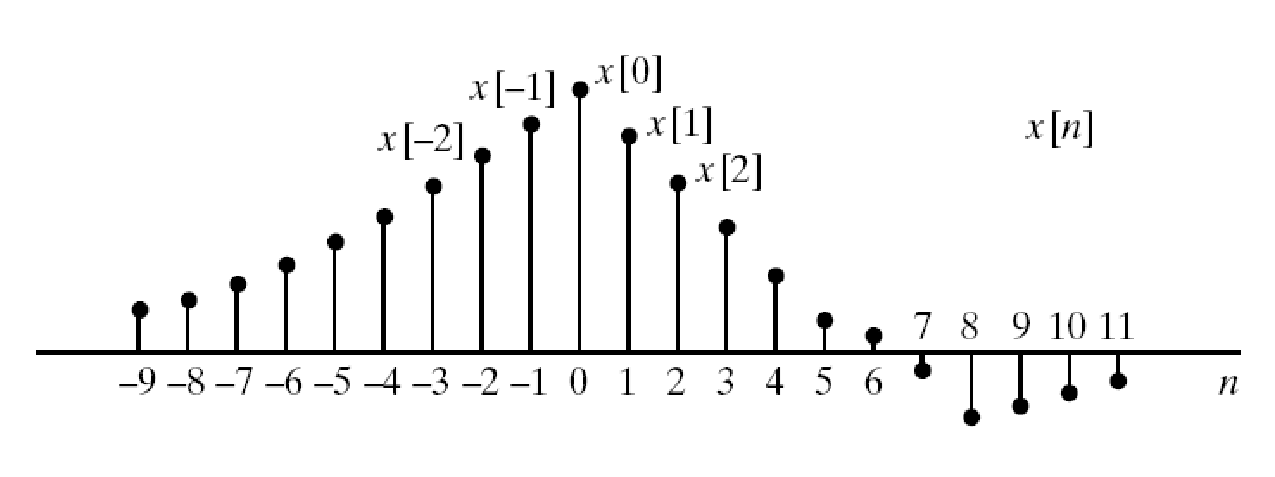
\includegraphics[width=\textwidth]{figs/2_1.eps}
   \end{center}
\end{slide}

\begin{slide}[toc=]{Amostragem de sinais contínuos}
\begin{itemize}
 \item Período de amostragem $T=125 \mu \text{s}$\\
    \begin{center}
       \onslide*{1}{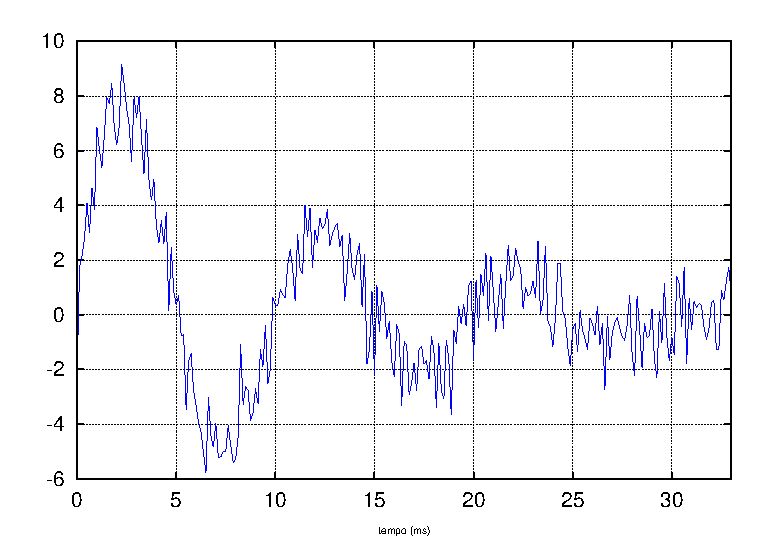
\includegraphics[width=0.7\textwidth]{figs/sCont.eps}}
      \onslide*{2}{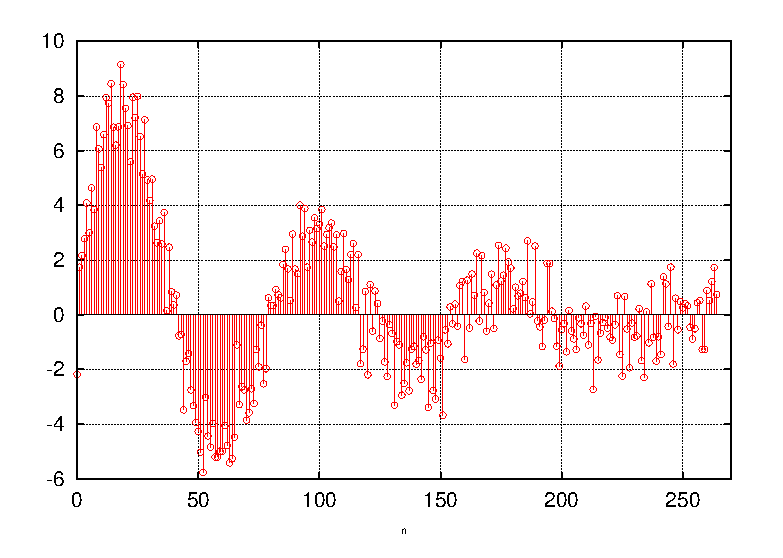
\includegraphics[width=0.7\textwidth]{figs/sDiscr.eps}}
      \onslide*{3}{$[ \begin{array}{ c c c c } -2,1738 &  1,7422 &  2,1658 &  \cdots \end{array} ]$}
    \end{center}
\end{itemize}
\end{slide}

\section[slide=true]{Sinais discretos: operações básicas}
\begin{slide}[toc=]{Operações básicas}
 \begin{itemize}
    \item
    \onslide*{1}{Sinais $x_1[n]$ e $x_2[n]$ \\
		 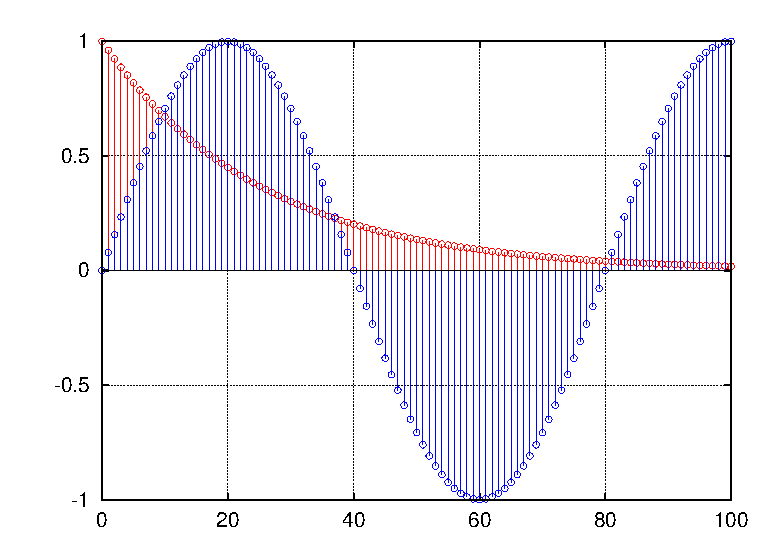
\includegraphics[width=0.7\textwidth]{figs/sX1eX2.eps}}
    \onslide*{2}{Soma de sinais: $x_1[n]+x_2[n]$
                          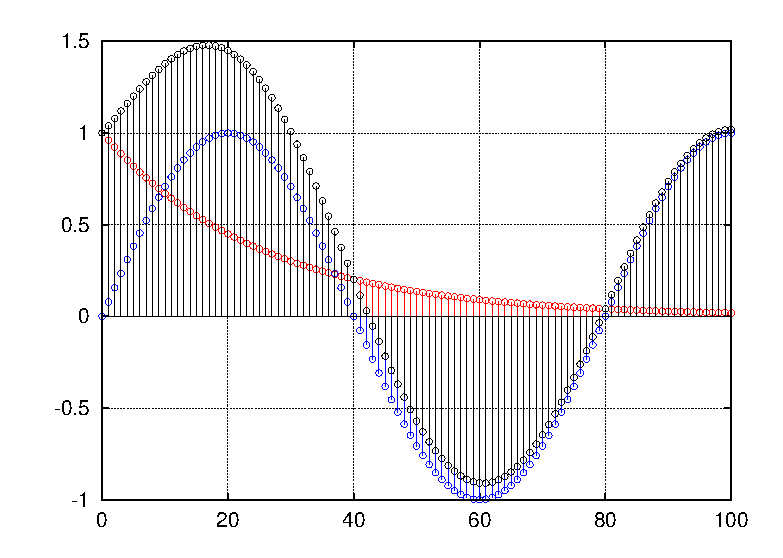
\includegraphics[width=0.7\textwidth]{figs/sX1maisX2.eps}} 
    \onslide*{3}{Multiplicação de sinais: $x_1[n]x_2[n]$
                          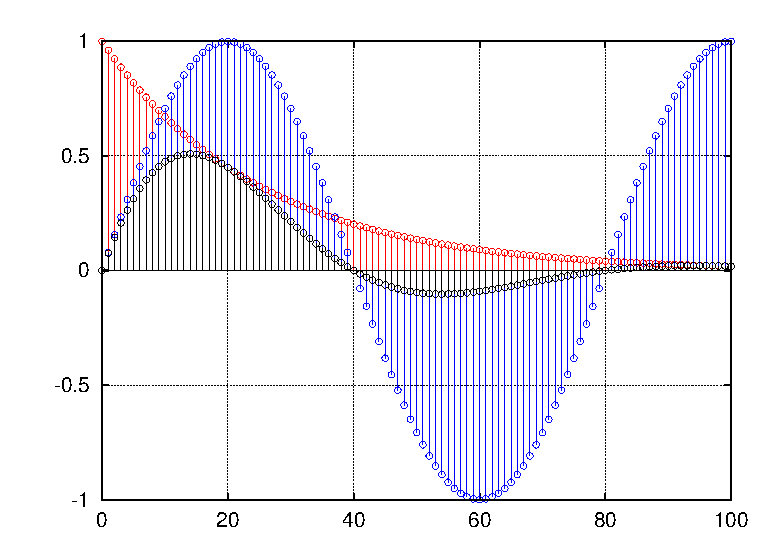
\includegraphics[width=0.7\textwidth]{figs/sX1vezesX2.eps} }
    \onslide*{4}{Multiplicação por escalar: $\alpha x[n]$ ($\alpha = 2$ e $0,5$)
                          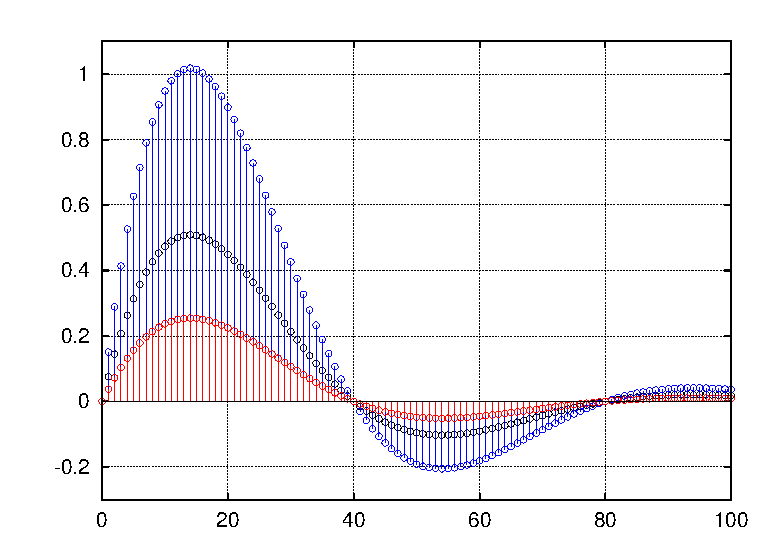
\includegraphics[width=0.7\textwidth]{figs/multConst.eps} }
    \onslide*{5}{Deslocamento: $x[n-n_o]$ ($n_o=20$)
                          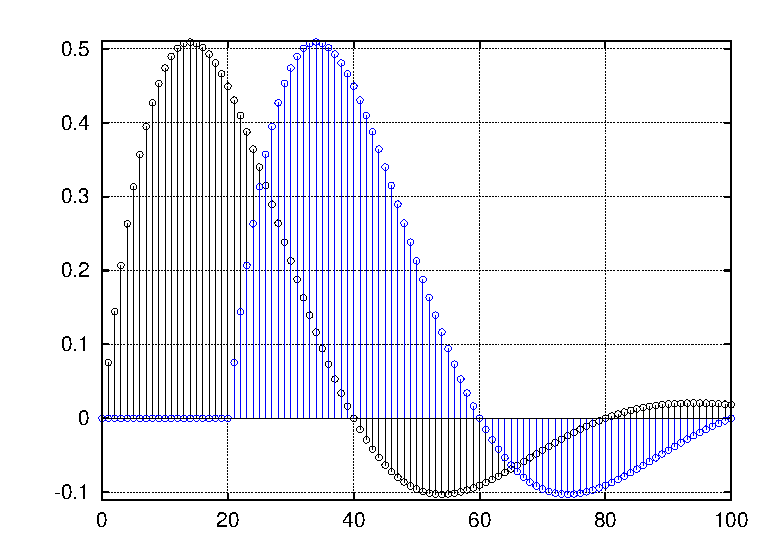
\includegraphics[width=0.7\textwidth]{figs/desloc.eps} }
  \end{itemize}
\end{slide}


\section[slide=true]{Sinais discretos: sequências básicas}
\begin{slide}[toc=]{Sequências básicas: impulso unitário}
\begin{itemize}
   \item Impulso unitário: 
      \onslide*{1-2}{
      \begin{equation*}
         \delta [n]=\begin{cases}
                  0, & n\neq 0,\\
                  1, & n=0,
                 \end{cases}
       \end{equation*}}
      \onslide*{2}{
      \begin{center}
        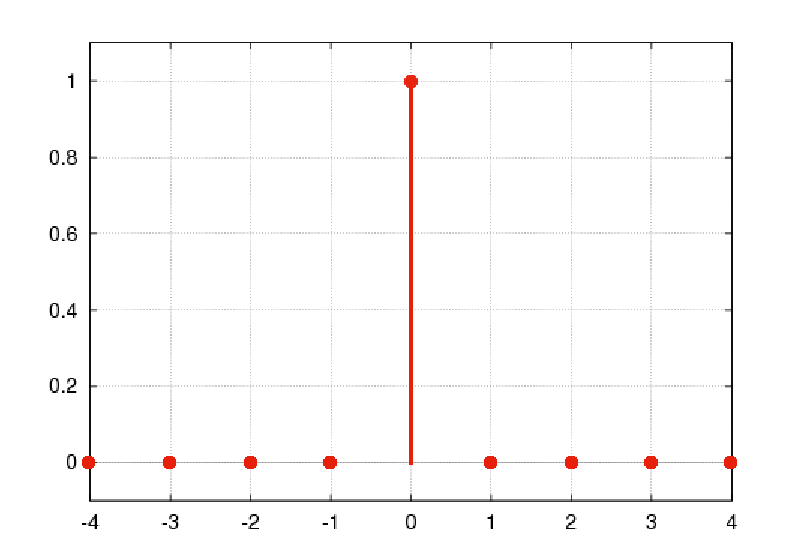
\includegraphics[width=0.5\textwidth]{figs/imp.eps}
      \end{center} }
     \onslide*{3}{
     \begin{center}
        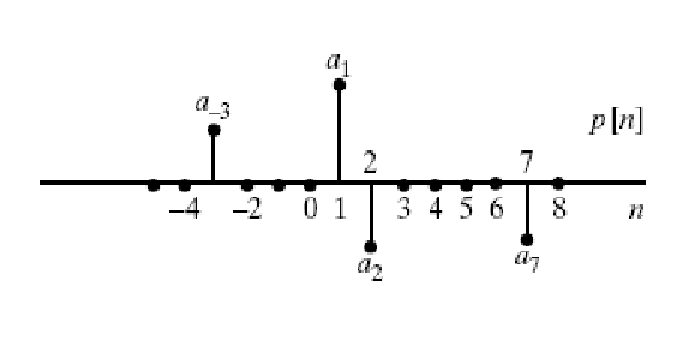
\includegraphics[width=0.5\textwidth]{figs/2_4.eps}
     \end{center} }
     \onslide*{4-11}{
     \begin{center}
        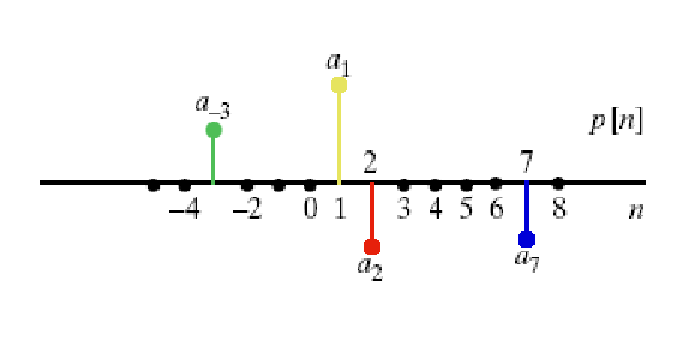
\includegraphics[width=0.5\textwidth]{figs/2_4a.eps}
     \end{center} }
     \onslide*{5}{
     \begin{center}
        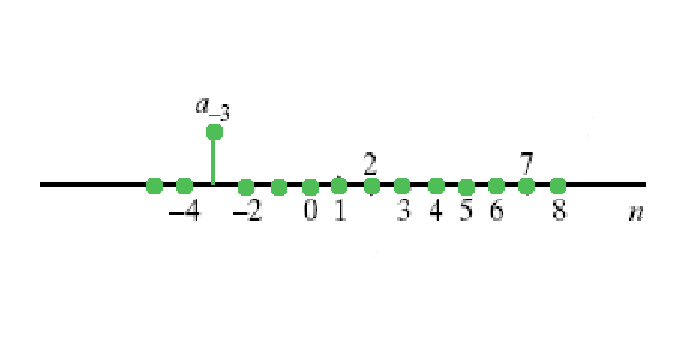
\includegraphics[width=0.5\textwidth]{figs/2_4b.eps}
     \end{center} }
     \onslide*{6}{
     \begin{center}
        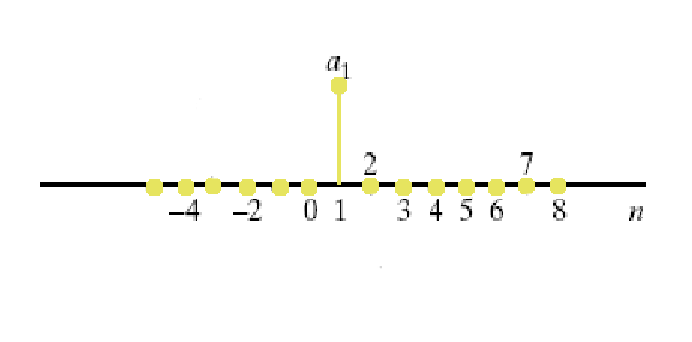
\includegraphics[width=0.5\textwidth]{figs/2_4c.eps}
     \end{center} }
     \onslide*{7}{
     \begin{center}
        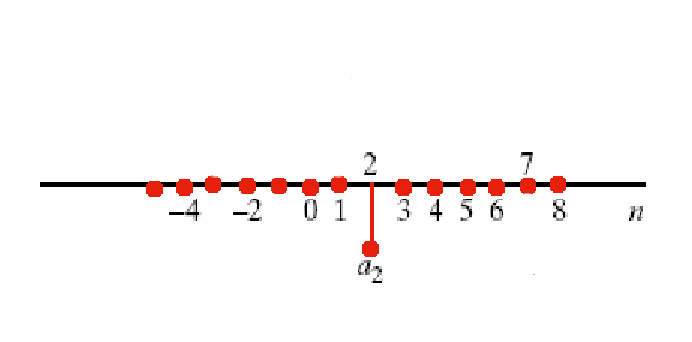
\includegraphics[width=0.5\textwidth]{figs/2_4d.eps}
     \end{center} }
     \onslide*{8}{
     \begin{center}
        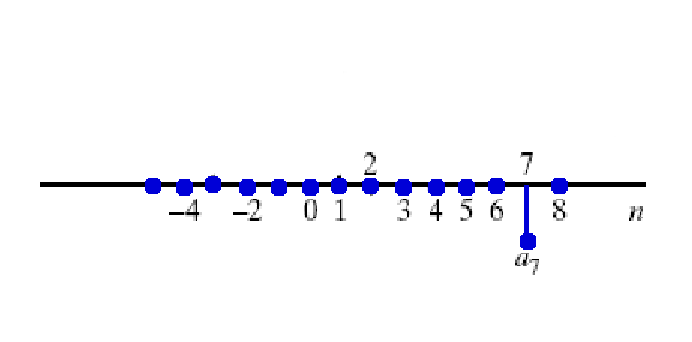
\includegraphics[width=0.5\textwidth]{figs/2_4e.eps}
     \end{center} }
     \onslide*{9}{
     \begin{align*}
        p[n] =& a_{-3}\delta [n+3]+a_{1}\delta [n-1]+\\
              &a_{2}\delta [n-2]+a_{7}\delta [n-7]
     \end{align*}}
     \onslide*{10}{
     \begin{align*}
        p[n] =& p[-3]\delta [n+3]+p[1]\delta [n-1]+\\
              & p[2]\delta [n-2]+p[7]\delta [n-7]
     \end{align*}}
     \onslide*{11}{
     \begin{equation*}
        \boxed{x[n]=\sum_{k=-\infty}^{\infty}x[k]\delta [n-k]}
     \end{equation*}}
    \end{itemize}
\end{slide} 

\begin{slide}[toc=]{Sequências básicas: degrau unitário}
\begin{itemize}
 \item Degrau unitário:
     \onslide*{1-2}{
     \begin{equation*}
      u[n]=\begin{cases}
                  1, & n \geq 0,\\
                  0, & n < 0,
                 \end{cases}
    \end{equation*}}
   \onslide*{2}{
   \begin{center}
     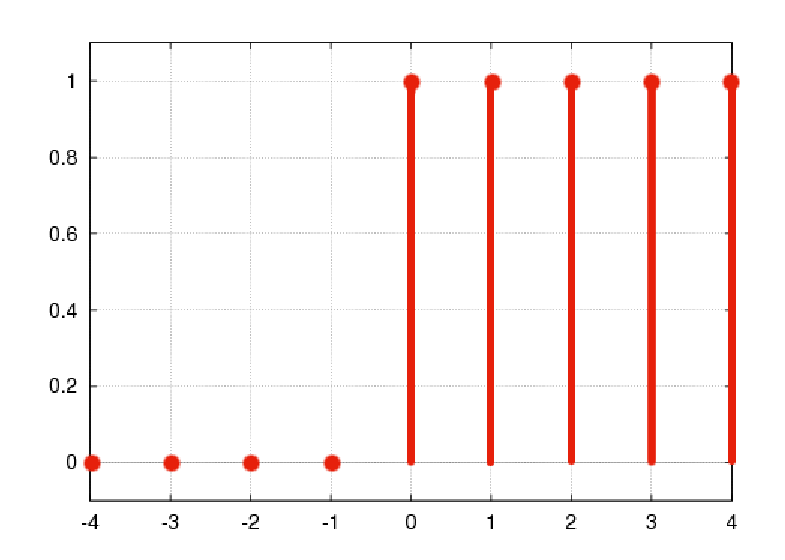
\includegraphics[width=0.5\textwidth]{figs/degrau.eps}
   \end{center} }
   \onslide*{3}{
      \begin{itemize}
         \item Identidades importantes:
         \begin{equation*}
            u[n]=\sum_{k=-\infty}^{n}\delta [k]
         \end{equation*}
         \begin{equation*}
            u[n]=\sum_{k=0}^{\infty}\delta [n-k]
         \end{equation*}
         \begin{equation*}
            \delta [n]=u[n]-u[n-1]
         \end{equation*}
      \end{itemize}
   }
\end{itemize}
\end{slide} 
\begin{slide}{Sequências básicas: sinal exponencial}
   \begin{itemize}
     \item Exponencial:
     \onslide*{1-3}{
     \begin{equation}
         x[n]=A\alpha^n
         \label{eq:expo}
     \end{equation}}
     \onslide*{2-3}{
     Em geral, $A$ e $\alpha$ são complexos:
     \begin{align}
         A &=|A|e^{j\phi} \label{eq:A}\\
         \alpha &= |\alpha|e^{j\omega_o}
         \label{eq:Alpha}
     \end{align}}
     \onslide*{3}{
     Substituindo (\ref{eq:A}) e (\ref{eq:Alpha}) em (\ref{eq:expo}),
      \begin{align*}
          x[n] & = |A||\alpha|^n e^{j(\omega_o n+\phi)}\\
               & = |A||\alpha|^n \left [  \text{cos}(\omega_o n+\phi) + j\text{sen}(\omega_o n+\phi)\right ]
      \end{align*}}
      \onslide*{4}{
         $x[n]=0,9^n$\\
         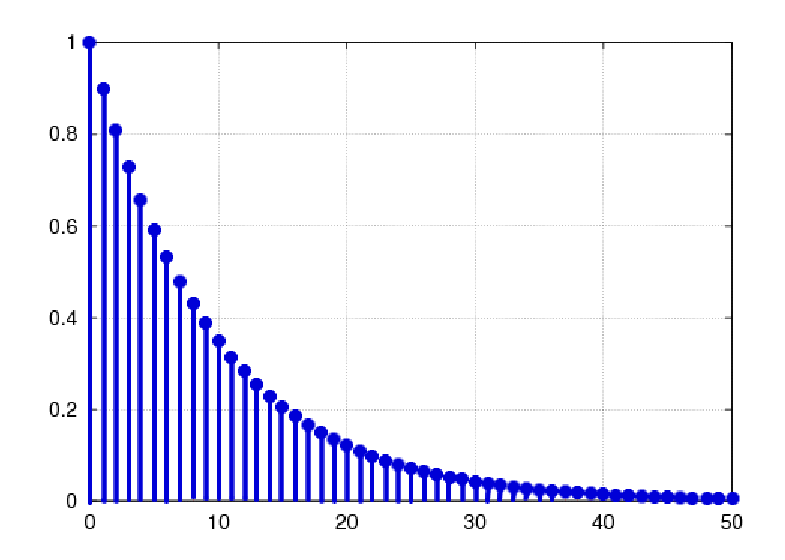
\includegraphics[width=0.7\textwidth]{figs/expo1.eps}}
       \onslide*{5}{
         $x[n]=1,1^n$\\
         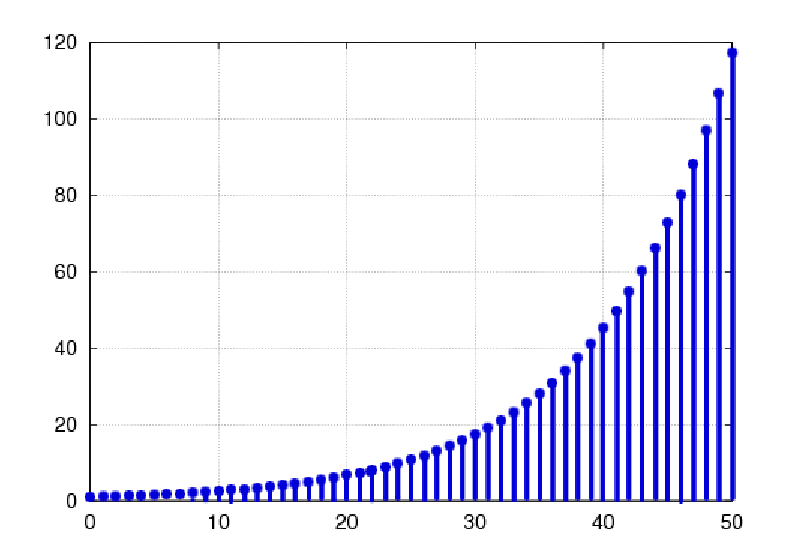
\includegraphics[width=0.7\textwidth]{figs/expo2.eps}}
       \onslide*{6}{
          $x[n]=\cos\left (\frac{\pi}{16}n \right )$\\
          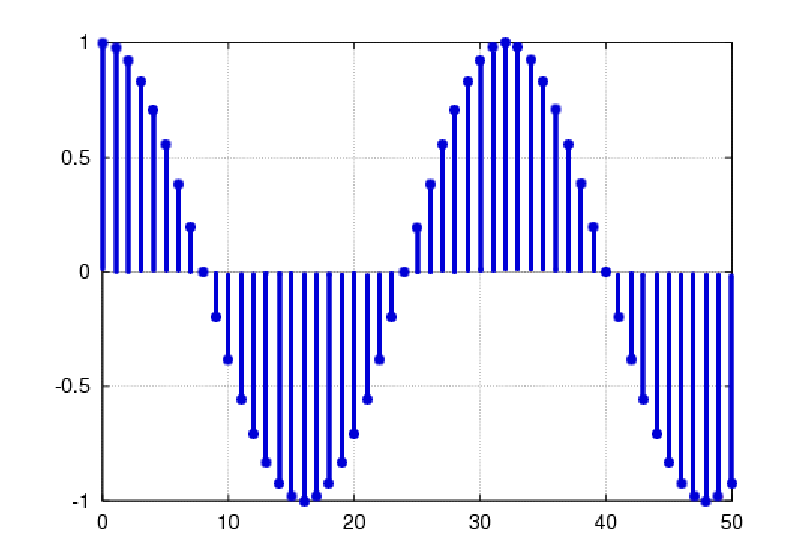
\includegraphics[width=0.7\textwidth]{figs/expo3.eps}}
       \onslide*{7}{
          $x[n]=0,7^n\cos\left (\frac{\pi}{16}n \right )$\\
          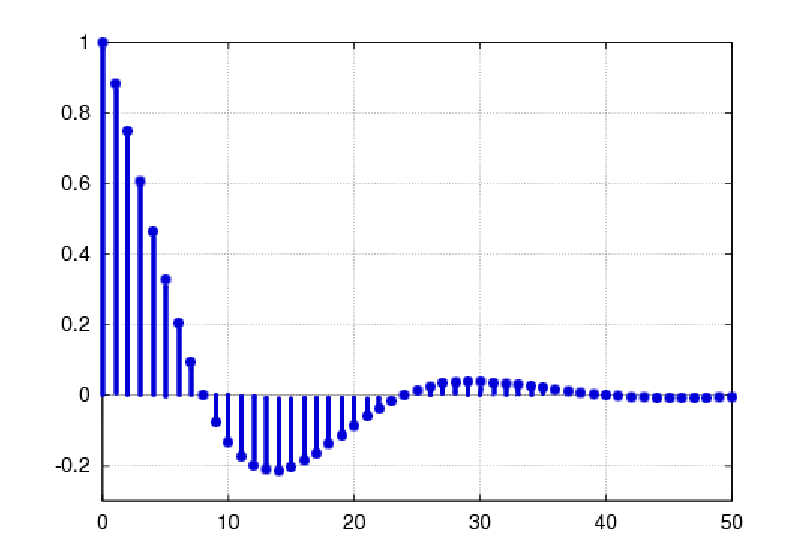
\includegraphics[width=0.7\textwidth]{figs/expo4.eps}}
       \onslide*{8}{
          $x[n]=1,1^n\cos\left (\frac{\pi}{16}n \right )$\\
          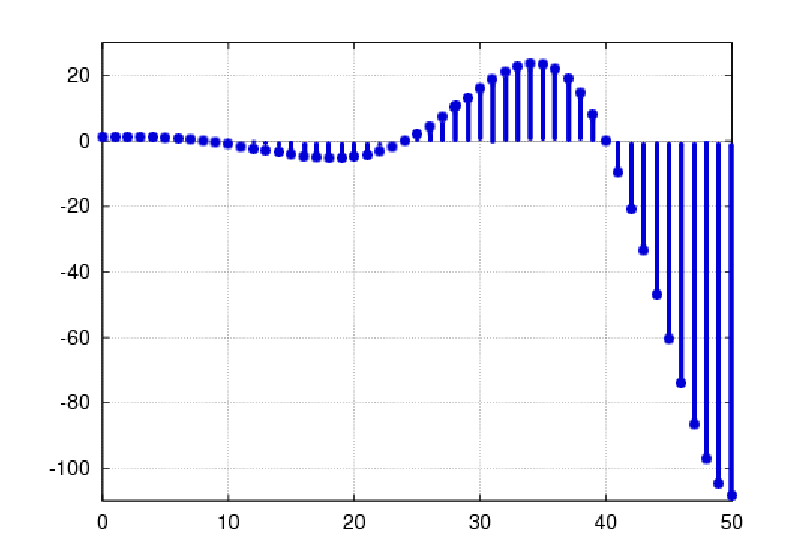
\includegraphics[width=0.7\textwidth]{figs/expo5.eps}}
       \end{itemize}
\end{slide}

 \begin{slide}{Sinais $e^{j\omega n}$: periodicidade em $\omega$ }
    \begin{itemize}
     \item <1-4> Considere um sinal do tipo $e^{j\omega_o n}$, onde $\omega_o$ representa um valor de ``frequência'' específico
     \item <2-4> O que acontece se formos aumentando o valor de $\omega_o$?
     \item <3-4> Chegará um momento em que 
        \begin{equation*}
             \omega_f = \omega_o + 2\pi
        \end{equation*}
        \begin{equation*}
        \begin{split}
           e^{j\omega_f n} & = e^{j(\omega_o + 2\pi)n} \\
                           &=e^{j\omega_o n}
         \end{split}
        \end{equation*}
        \begin{itemize}
           \item <4>\textcolor{red}{Não há distinção entre as ``frequências'' $\omega_o$ e $\omega_o+2\pi$}
     \end{itemize}
   \end{itemize}
 \end{slide}
 
 
\begin{slide}{Sinais $e^{j\omega n}$: periodicidade em $\omega$ }
   \begin{itemize}
    \item %Periodicidade em $\omega$:
    \onslide*{1}{$\omega_1 = 0$; $\omega_2 = 2\pi$ 
    \begin{center}
     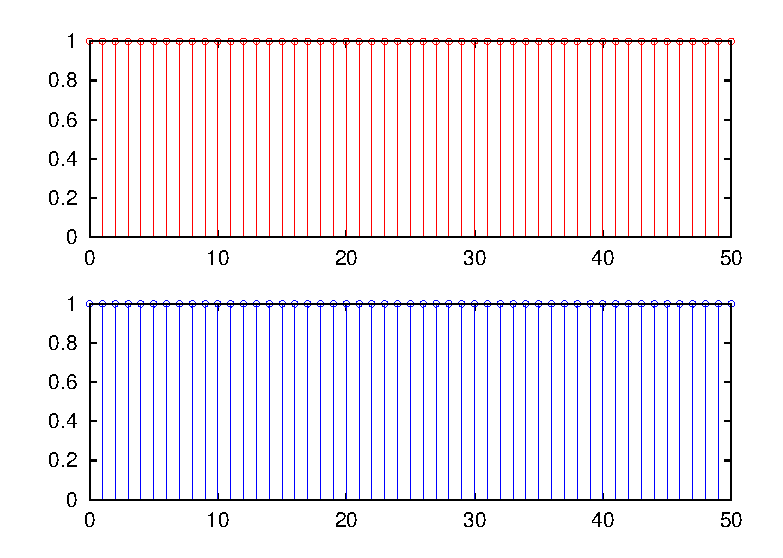
\includegraphics[width=0.7\textwidth]{figs/perfreq01.eps}
    \end{center}}
    \onslide*{2}{$\omega_1 = \frac{\pi}{4}$; $\omega_2 = \frac{9\pi}{4}$ 
    \begin{center}
     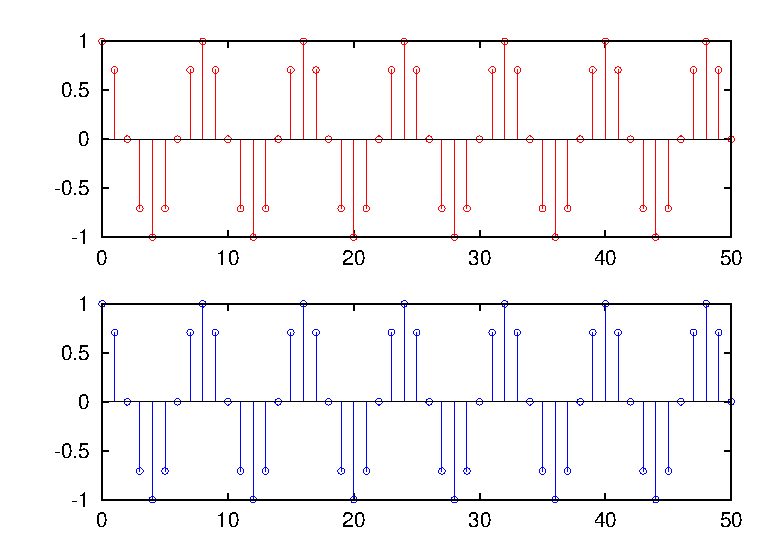
\includegraphics[width=0.7\textwidth]{figs/perfreq02.eps}
    \end{center}}
    \onslide*{3}{$\omega_1 = \frac{\pi}{3}$; $\omega_2 = \frac{7\pi}{3}$ 
    \begin{center}
     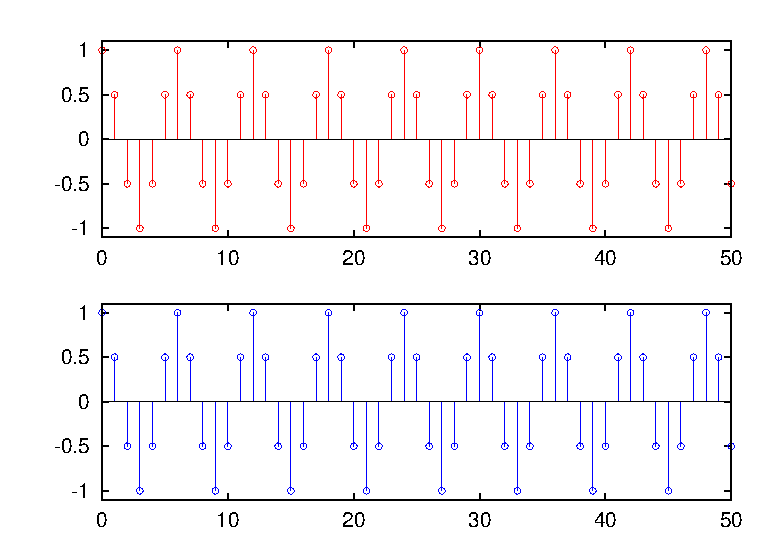
\includegraphics[width=0.7\textwidth]{figs/perfreq03.eps}
    \end{center}}
   \onslide*{4}{$\omega_1 = \frac{\pi}{1,1}$; $\omega_2 = \frac{3,2\pi}{1,1}$ 
    \begin{center}
     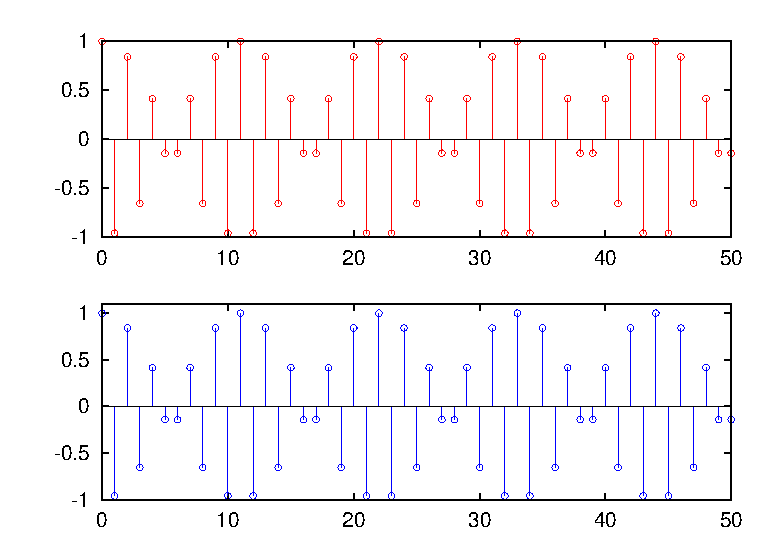
\includegraphics[width=0.7\textwidth]{figs/perfreq04.eps}
    \end{center}}
   \onslide*{5}{O deslocamento de $2\pi$ faz com que se volte ao ``mesmo ponto''
    \begin{center}
     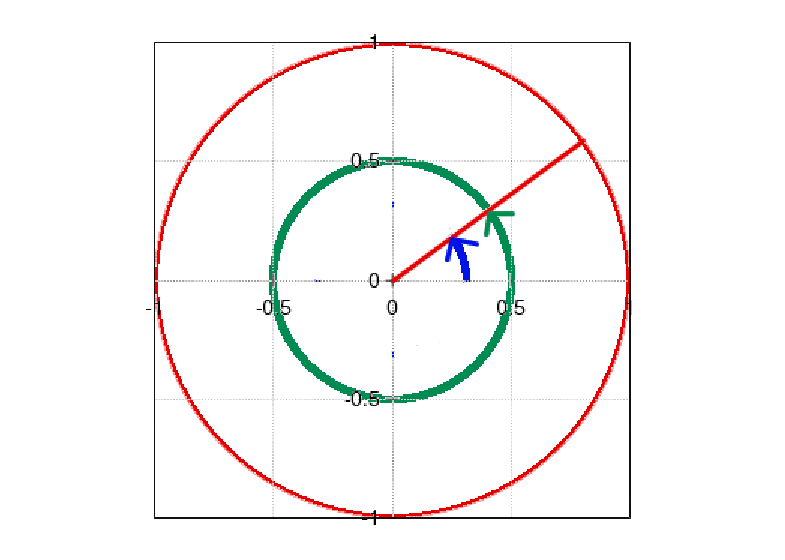
\includegraphics[width=0.7\textwidth]{figs/perfreq_circ.eps}
    \end{center}}
   \end{itemize}
\end{slide}
 
\begin{slide}{Sinais $e^{j\omega n}$: periodicidade em $n$ }
   \begin{itemize}
    \item <1-3> Considerando um sinal do tipo $e^{j\omega_o n}$, onde $\omega_o$ representa um valor de ``frequência'' específico
     \item <2-3> Que condições tal sinal deve possuir para ser periódico em $n$?
     \item <3-3> Se $e^{j\omega_o n}$ é periódico em $n$ com período $N$,
        \begin{align*}
           e^{j\omega_o n} &= e^{j\omega_o (n+N)}\\
                           &= e^{j\omega_o n} e^{j\omega_o N}\\
        %\end{align*}
        %\onslide*{4}{
        %\begin{align*}
             \omega_o N &= k2\pi, \quad N, k \in \mathbb{Z}\\
               \omega_o &= \frac{k2\pi}{N} \Rightarrow \frac{\omega_o}{2\pi} = \frac{k}{N}\quad k=0,1,\ldots, N-1
         \end{align*}%}
     %Há, assim, um número \textcolor{red}{finito} de sinais periódicos $e^{j\omega_o}$ distintos: $k=0,1,\ldots, N-1$
%     \end{itemize}
%  \end{itemize}
\end{itemize}
\end{slide} 

\begin{note}{O número de sinais exponenciais periódicos}
   Há, assim, um número \textcolor{red}{finito} de sinais periódicos $e^{j\omega_o}$ distintos: $k=0,1,\ldots, N-1$
\end{note}


\begin{slide}{Sinais $e^{j\omega n}$: periodicidade em $n$ }
   \begin{itemize}
    \item Exemplos:
    \onslide*{1}{
     $\omega = \frac{\pi}{7}$
    \begin{center}
     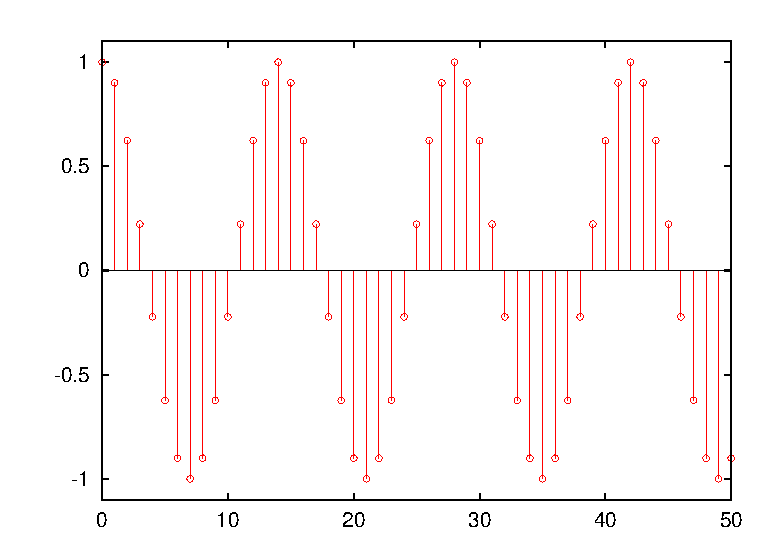
\includegraphics[width=0.7\textwidth]{figs/perfn01.eps}
    \end{center}}
    \onslide*{2}{
     $\omega = 0,45$ 
    \begin{center}
     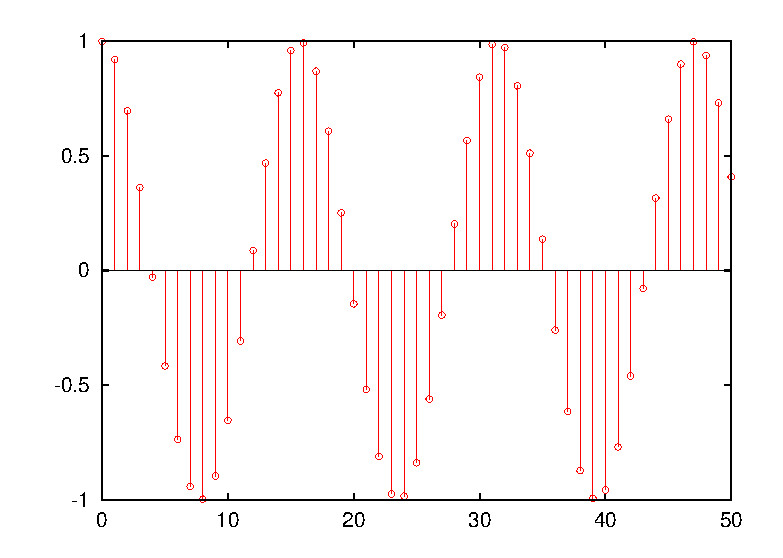
\includegraphics[width=0.7\textwidth]{figs/perfn02.eps}
    \end{center}}
   \end{itemize}
\end{slide}

\section[slide=true]{Sistemas discretos: definições e propriedades}
\begin{slide}{Definições}
   \begin{itemize}
   \item <1->Mapeamento entre entrada e saída de um sistema
    \setlength{\unitlength}{1cm}
    \begin{center}
    \begin{picture}(4,1)
      \thicklines
      \put( 0, 0.5 ) {\vector(1,0){1}}
      \put( 1, 0 ) {\framebox( 2, 1){T\{$\bullet$\}}}
      \put( 3, 0.5 ) {\vector(1,0){1}}
      
      \put(0.2,0){$x$}
      \put(3.2,0){$y$}
      
    \end{picture}
    \end{center}

    \item <2->Sistemas sem memória: saída atual $y[n]$ depende somente da entrada atual $x[n]$
    \item <3->Sistemas invariantes: 
    \begin{align*}
        y_1[n] &=\text{T}\{x_1[n]\}\\
        y_2[n] &=\text{T} \{x_2[n]\} \\
               &=\text{T} \{x_1[n-n_o]\}= y_1[n-n_o]\\
      \end{align*}
  \end{itemize}
\end{slide}

\begin{slide}{Invariância: exemplos}
   \begin{itemize}
   \item Sistemas invariantes -- Exemplo:
   \onslide*{1} {
   \begin{center}
     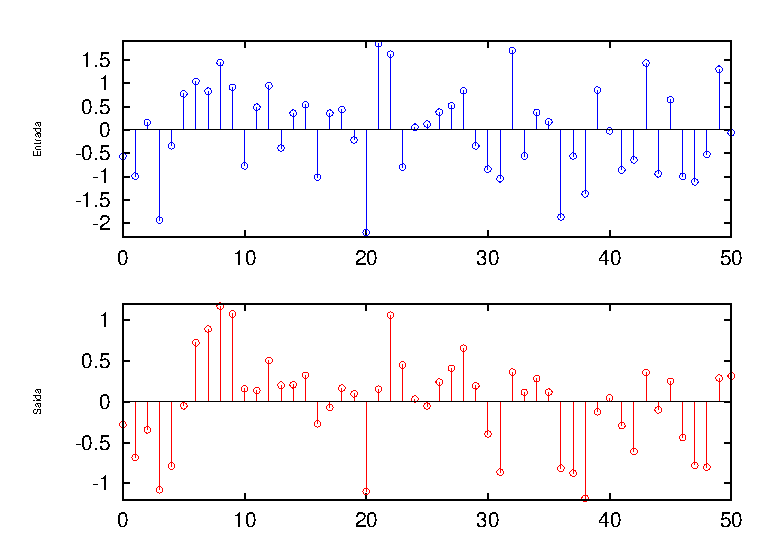
\includegraphics[width=0.7\textwidth]{figs/invariante01.eps}
    \end{center}}
   \onslide*{2} {
   \begin{center}
     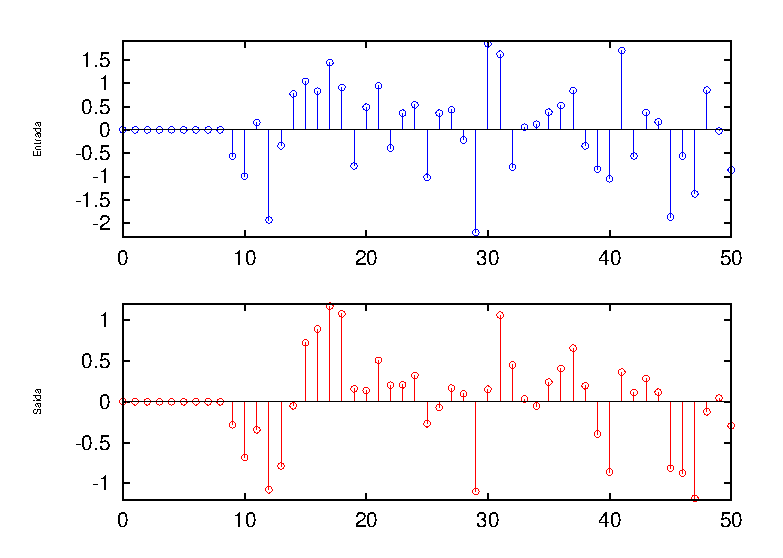
\includegraphics[width=0.7\textwidth]{figs/invariante02.eps}
    \end{center}}
   \end{itemize}
\end{slide} 

\begin{slide}{Causalidade e estabilidade}
   \begin{itemize}
    \item <1->Causalidade: a saída $y[n_o]$ depende das entradas $x[n]$, onde $n \leq n_o$
    \item <2>Estabilidade: BIBO (\textit{bounded-input bounded-output})\\
    \begin{align*}
       |x[n]| \leq B_x < \infty, \quad \forall n\\
       |y[n]| \leq B_y < \infty, \quad \forall n
    \end{align*}

  \end{itemize}
\end{slide}


\begin{slide}{Sistemas lineares}
   \begin{itemize}
       \item <1->Princípio da homogeneidade:
       \begin{equation*}
        \text{T}\{\alpha x[n]\} = \alpha \text{T}\{ x[n]\}
       \end{equation*}
       \item <2->Princípio da aditividade:
       \begin{equation*}
           \text{T}\{x_1[n]+x_2[n]\} = \text{T}\{x_1[n]\} + \text{T}\{x_2[n]\}
       \end{equation*}
       \item <3>\textcolor{red}{Princípio da superposição:}
       \begin{equation*}
     \text{T}\{\alpha x_1[n] + \beta x_2[n] \}= \alpha \text{T}\{x_1[n]\} + \beta \text{T}\{x_2[n]\}
    \end{equation*}
    \end{itemize} 
\end{slide}

\section[slide=true]{Sistemas discretos lineares e invariantes}
\begin{slide}{Mapeamento entre entrada e saída}
   \begin{itemize}
    \item <1->Resposta $y[n]$ de um sistema LI ao sinal $x[n]$
    \begin{align*}
        y[n]&=\text{T}\left \{ x[n] \right \}\\
            &=\text{T}\left \{ \sum_{k=-\infty}^{\infty}x[k]\delta [n-k] \right \}.
    \end{align*}
     \item <2-> Usando o \emph{princípio da superposição},
     \begin{align*}
        y[n]&=\sum_{k=-\infty}^{\infty}x[k]\text{T}\left \{ \delta [n-k] \right \}\\
            &=\sum_{k=-\infty}^{\infty}x[k]h_k[n].
     \end{align*}
   \end{itemize}
\end{slide}


\begin{slide}{Mapeamento entre entrada e saída}
   \begin{itemize}
    \item <1->Considerando o sistema invariante,
    \begin{align*}
        y[n]&=\sum_{k=-\infty}^{\infty}x[k]h_k[n]\\
            &=\sum_{k=-\infty}^{\infty}x[k]h[n-k].
     \end{align*}
     \onslide*{2}{Soma (somatório) de convolução:
     \begin{equation*}
         \boxed{y[n]=\sum_{k=-\infty}^{\infty}x[k]h[n-k]}
     \end{equation*}}
   \end{itemize}
\end{slide}

\begin{slide}{Convolução}
   \begin{equation*}
      y[n]=x[n]*h[n]=\sum_{k=-\infty}^{\infty}x[k]h[n-k]
   \end{equation*}
   \begin{center}
      \onslide*{1}{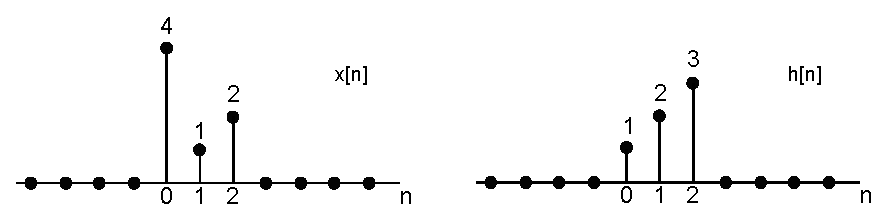
\includegraphics[width=0.8\textwidth]{figs/doissinais.eps}}
      \onslide*{2}{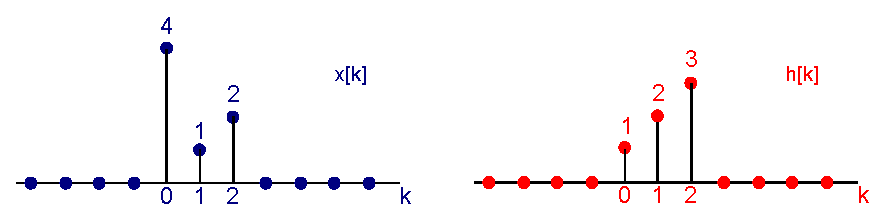
\includegraphics[width=0.8\textwidth]{figs/doissinais2.eps}}
      \onslide*{3}{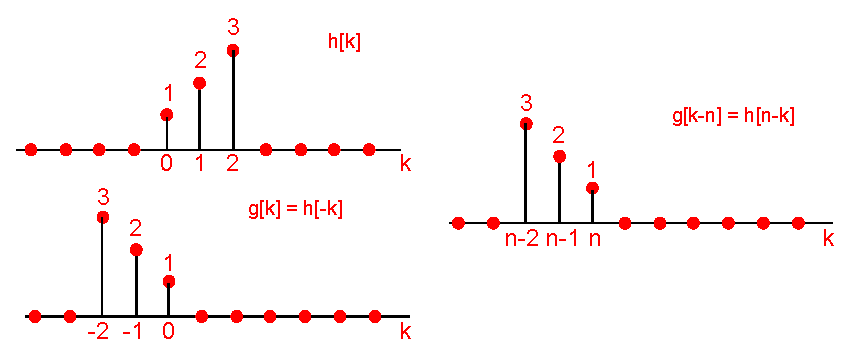
\includegraphics[width=0.8\textwidth]{figs/hs.eps}}
      \onslide*{4}{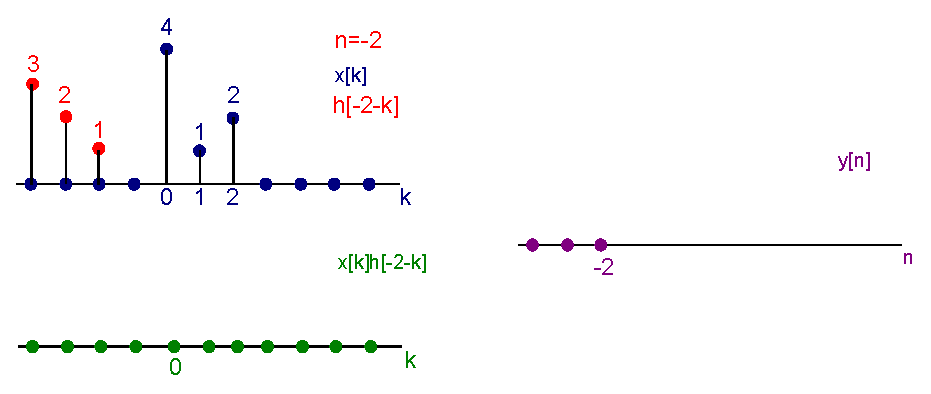
\includegraphics[width=0.8\textwidth]{figs/step1.eps}}
      \onslide*{5}{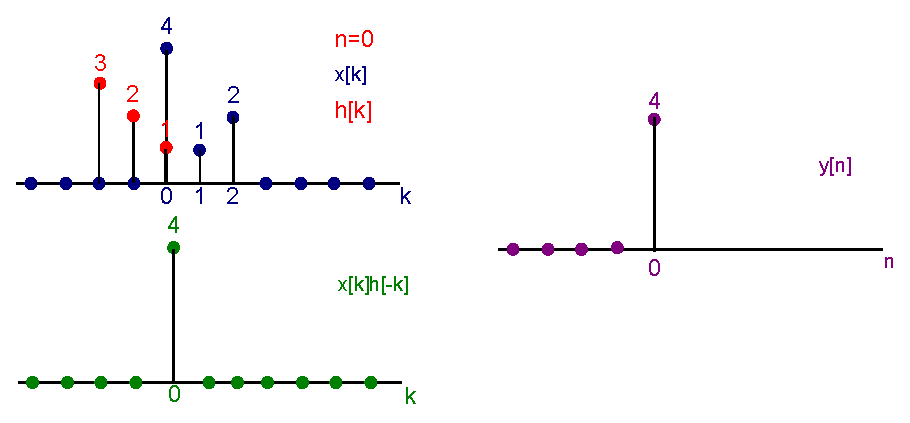
\includegraphics[width=0.8\textwidth]{figs/step2.eps}}
      \onslide*{6}{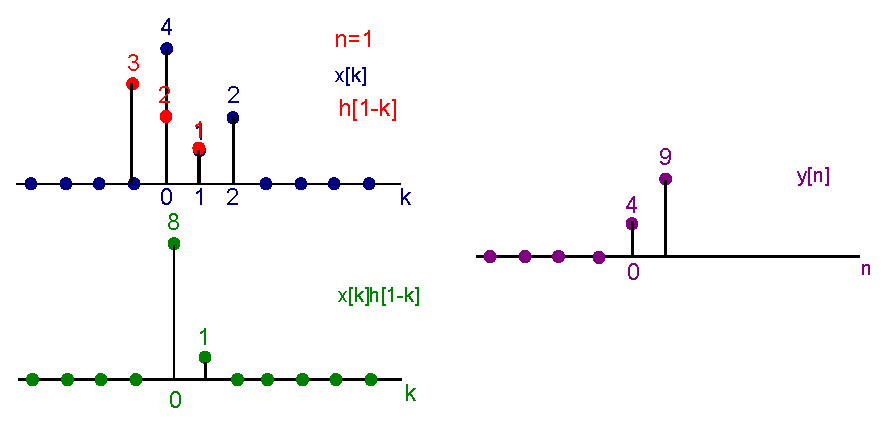
\includegraphics[width=0.8\textwidth]{figs/step3.eps}}
      \onslide*{7}{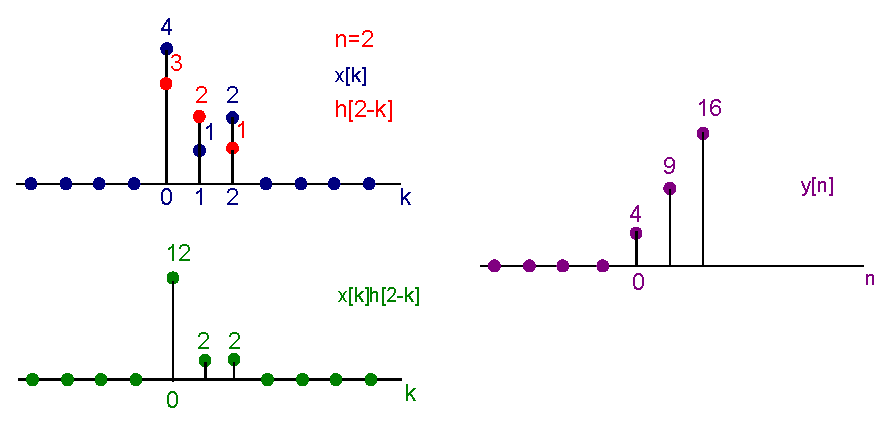
\includegraphics[width=0.8\textwidth]{figs/step4.eps}}
      \onslide*{8}{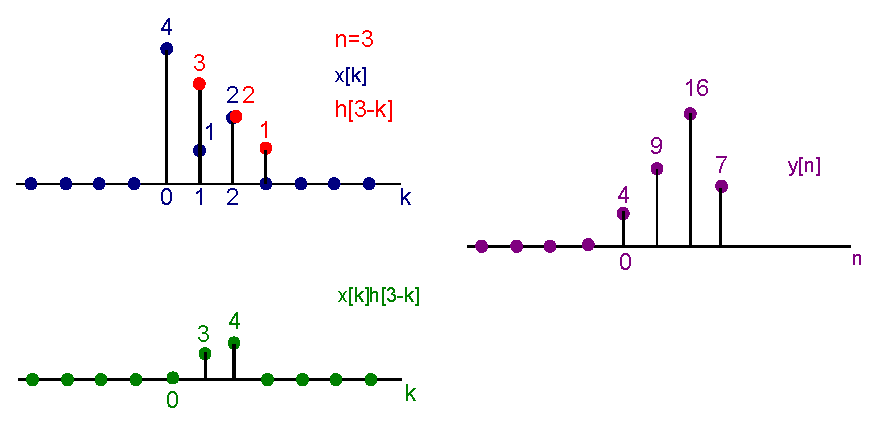
\includegraphics[width=0.8\textwidth]{figs/step5.eps}}
      \onslide*{9}{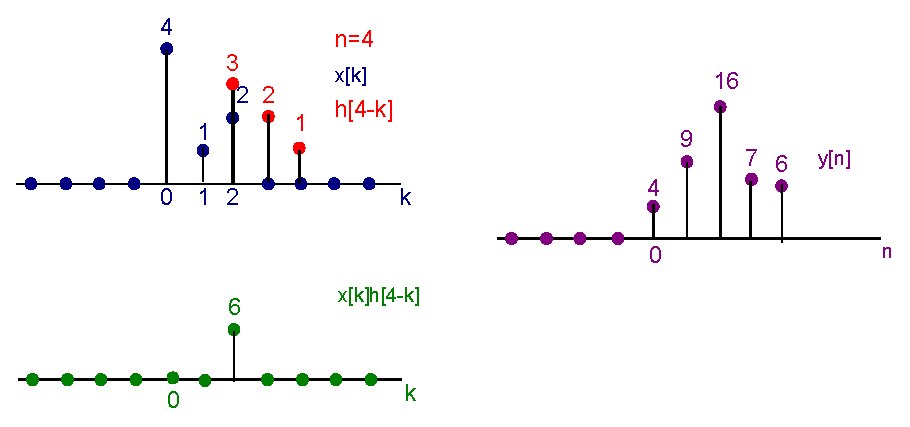
\includegraphics[width=0.8\textwidth]{figs/step6.eps}}
      \onslide*{10}{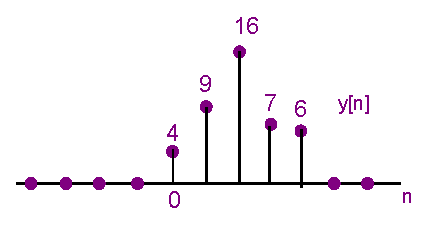
\includegraphics[width=0.8\textwidth]{figs/y.eps}}
   \end{center}
\end{slide}

\section[slide=true]{Propriedades dos sistemas LI}
\begin{slide}{Comutatividade}
   \begin{itemize}
    \item $x[n]\ast h[n] = h[n]\ast x[n]$
    \item Sistemas em cascata:
    \setlength{\unitlength}{1cm}
    \begin{center}
    \begin{picture}(7,3.5)
      \thicklines
      \put( 0, 0.5 ) {\vector(1,0){1}}
      \put( 1, 0 ) {\framebox( 5, 1){$h_1[n]\ast h_2[n]$}}
      \put( 6, 0.5 ) {\vector(1,0){1}}
      
      \put(0.3,0){$x$}
      \put(6.3,0){$y$}
      
      \put( 0, 1.75 ) {\vector(1,0){1}}
      \put( 1, 1.25 ) {\framebox( 2, 1){$h_2[n]$}}
      \put( 3, 1.75 ) {\vector(1,0){1}}
      \put( 4, 1.25 ) {\framebox( 2, 1){$h_1[n]$}}
      \put( 6, 1.75 ) {\vector(1,0){1}}
      
      \put(0.3,1.25){$x$}
      \put(6.3,1.25){$y$}
      
      \put( 0, 3 ) {\vector(1,0){1}}
      \put( 1, 2.5 ) {\framebox( 2, 1){$h_1[n]$}}
      \put( 3, 3 ) {\vector(1,0){1}}
      \put( 4, 2.5) {\framebox( 2, 1){$h_2[n]$}}
      \put( 6, 3 ) {\vector(1,0){1}}
      
      \put(0.3,2.5){$x$}
      \put(6.3,2.5){$y$}
      
    \end{picture}
    \end{center}
   \end{itemize}
\end{slide}


\begin{slide}{Distributividade}
   \begin{itemize}
    \item $x[n]\ast\left ( h_1[n]+h_2[n]\right ) = x[n]\ast h_1[n]+ x[n]\ast h_2[n]$
    \item Sistemas em paralelo:
    \setlength{\unitlength}{1cm}
    \begin{center}
    \begin{picture}(7,3.5)
      \thicklines
      \put( 0, 0.5 ) {\vector(1,0){1}}
      \put( 1, 0 ) {\framebox( 5, 1){$h_1[n]+ h_2[n]$}}
      \put( 6, 0.5 ) {\vector(1,0){1}}
      
      \put(0.3,0){$x$}
      \put(6.3,0){$y$}
      %------------------------
      \put(2.5, 1.25){\framebox(2,1){$h_2[n]$}}
      \put(2.5, 2.5){\framebox(2,1){$h_1[n]$}}
      \put(1.5, 1.75){\vector(1,0){1}}
      \put(1.5, 3){\vector(1,0){1}}
      \put(1.5, 3){\line(0,-1){1.25}}
      \put(4.5, 1.75){\line(1,0){1}}
      \put(4.5, 3){\line(1,0){1}}
      
      \put(5.5,2.375){\circle{0.5}}
      \put(5.75,2.375){\vector(1,0){1}}
      \put(0.5,2.375){\vector(1,0){1}}
      \put(5.5,1.75){\vector(0,1){0.375}}
      \put(5.5,3){\vector(0,-1){0.375}}
      \put(5.35,2.275){+}
      
      \put(0.8,1.875){$x$}
      \put(6.05,1.875){$y$}
    \end{picture}
    \end{center}
   \end{itemize}
\end{slide}

\begin{slide}{Causalidade}
   \begin{itemize}
      \item Causalidade: \\
            Um sistema LI é causal se\begin{equation*} h[n] = 0, \quad n<0 \end{equation*}
            Por quê?
   \end{itemize}
\end{slide}

\begin{slide}{Estabilidade}
   \begin{itemize}
    \item Um sistema LI é estável se
    \begin{equation*}
        S = \sum_{n=-\infty}^{\infty}|h[n]|<\infty
    \end{equation*}
    
    A resposta do sistema ao impulso é \textcolor{red}{absolutamente somável} (condição suficiente
    e necessária para estabilidade).\pause
    \begin{align*}
       |y[n]|&=\left | \sum_{k=-\infty}^{\infty} h[k]x[n-k]\right |\\
             &\leq \sum_{k=-\infty}^{\infty} |h[k]||x[n-k]|
    \end{align*}
   \end{itemize}
\end{slide}

\begin{slide}{Estabilidade}
    Como $|x[n]|\leq B_x < \infty$ (a entrada é limitada), então 
    \begin{equation*}|y[n]|\leq \sum_{k=-\infty}^{\infty} |h[k]||x[n-k]|\leq B_x\sum_{k=-\infty}^{\infty} |h[k]|\end{equation*}\pause
    
    Logo, para que a saída seja limitada $|y[n]|\leq B_y < \infty$,
    \begin{align*}|y[n]|&\leq B_x\sum_{k=-\infty}^{\infty} |h[k]| < \infty\\
                        &\Rightarrow \boxed{\sum_{k=-\infty}^{\infty} |h[k]| < \infty}
    \end{align*}
\end{slide}

\section[slide=true]{Equações de diferenças}
\begin{slide}[toc=]{Definições}
   \begin{itemize}
    \item Equação de diferenças de $N$-ésima ordem e coeficientes constantes:
    \begin{equation*}
       \sum_{ k = 0 }^{ N } a_k y[ n - k ]=\sum_{ m = 0 }^{ M } b_m x[ n - m ],
    \end{equation*}
    onde $x[n]$ e $y[n]$ são entrada e saída do sistema.
   \end{itemize}
\end{slide}

\begin{slide}[toc=]{Exemplos}
   \begin{itemize}
   \item Acumulador
    \begin{equation*}
       %\begin{split}
         y[n] = \sum_{ k = -\infty}^{n} x[k]= y[n-1] + x[n]
       %\end{split}
   \end{equation*}\pause
    \item Média móvel
    \begin{align*}
         y[n] &= \frac{1}{M_2+1}\sum_{ k = 0}^{M_2} x[n-k]\\
         h[n] &= \frac{1}{M_2+1}\left ( u[n] - u[n-M_2-1] \right )\\
              &= \frac{1}{M_2+1}\left ( \delta[n] - \delta[n-M_2-1] \right )\ast u[n]
    \end{align*}
   \end{itemize}
\end{slide}


\begin{slide}[toc=]{Resolução}
   \begin{itemize}
      \item Pode-se rescrever a eq. de diferenças como
      \begin{equation*}
         \sum_{ k = 0 }^{ N } a_k y[ n - k ]-\sum_{ m = 0 }^{ M } b_m x[ n - m ]=0
      \end{equation*}\pause
      \item Há dois tipos de solução:
      \begin{itemize}
         \item Solução particular ($y_p[n]$): quando $x[n]\neq 0$
         \item Solução homogênea ($y_h[n]$): quando $x[n]= 0$
      \end{itemize}
   \end{itemize}
\end{slide}

\begin{slide}[toc=]{Solução particular e homogênea}
   \begin{itemize}
      \item Solução particular ($x[n]\neq 0$)
      \begin{equation*}
         \sum_{ k = 0 }^{ N } a_k y_p[ n - k ]-\sum_{ m = 0 }^{ M } b_m x[ n - m ]=0
      \end{equation*}\pause
      \item Solução homogênea ($x[n]=0$)
      \begin{equation*}
         \sum_{ k = 0 }^{ N } a_k y_h[ n - k ]=0
      \end{equation*}
   \end{itemize}
\end{slide}

\begin{slide}[toc=]{Solução completa}
   \begin{itemize}
      \item A soma das soluções particular e homogênea também é solução da equação de diferenças
      \begin{equation*}
         \sum_{ k = 0 }^{ N } a_k \{y_p[ n - k ]+y_h[ n - k ]\}-\sum_{ m = 0 }^{ M } b_m x[ n - m]=0
      \end{equation*}\pause
      \item Graus de liberdade ($N$): 
      \begin{itemize}
         \item Depende de $N$ constantes arbitrárias
         \item Necessita de $N$ condições iniciais auxiliares
      \end{itemize}
   \end{itemize}
\end{slide}

\begin{slide}[toc=]{Determinação da solução homogênea}
   \begin{itemize}
      \item A solução homogênea é da forma
      \begin{equation*}
         y_h[n]=\sum_{m=1}^N A_m z_m^n
      \end{equation*}
      \item Assim, os números complexos $z_m$ devem ser raízes do polinômio
      \begin{equation*}
         \sum_{k=0}^N a_k z^{-k}
      \end{equation*}
      \item Após a determinação dos $z_m$, as constantes $A_m$ devem ser calculadas com o auxílio 
      de $N$ condições auxiliares.
   \end{itemize}
\end{slide}

\begin{slide}[toc=]{Discussão}
   \begin{itemize}
      \item Para um sistema cuja entrada e saída satisfazem uma equação de 
      diferenças linear com coeficientes constantes:
      \begin{itemize}
         \item A saída para uma dada entrada não é única, depende de condições auxiliares
         \item A linearidade, a invariância e a causalidade dependerão das condições auxiliares 
         (sistema em repouso ou não)
      \end{itemize}
      \item Caso especial: $N=0$
      \begin{itemize}
         \item Não há necessidade de recursão, nem de condições iniciais
         \item A saída é dada pela expressão
         \begin{equation*}
            y[n]=\sum_{k=0}^M\left (\frac{b_k}{a_0}\right )x[n-k]
         \end{equation*}
      \end{itemize}
   \end{itemize}
\end{slide}

\begin{slide}[toc=]{Discussão}
   \begin{itemize}
      \item Caso especial: $N=0$
      \begin{itemize}
         \item Resposta ao impulso finita (FIR)
         \begin{equation*}
            y[n]=\begin{cases}
                    \frac{b_k}{a_0}, & 0\leq n \leq M,\\
                    0              , & \text{caso contrário}
                 \end{cases}
         \end{equation*}
      \end{itemize}
   \end{itemize}
\end{slide}


\section[slide=true]{Representação em frequência}
 \begin{slide}[toc=]{Auto-funções}
\begin{itemize}
 \item Funções exponenciais complexas como ``auto-funções'' de um sistema LI
 \begin{align*}
   x[n]&=e^{j\omega n}\\
   y[n]&=\sum_{k=-\infty}^{\infty}h[k]e^{j\omega (n-k)}\\
       &=e^{j\omega n}\left [\sum_{k=-\infty}^{\infty}h[k]e^{-j\omega k} \right ]\\
       &= H(e^{j\omega})e^{j\omega n}
 \end{align*}%}
 $H(e^{j\omega})$: \textcolor{red}{resposta em frequência do sistema.}
\end{itemize}
\end{slide}

\begin{slide}[toc=]{Exemplos}
\begin{itemize}
   \item Ache a $H(e^{j\omega})$ do sistema $y[n]=x[n-n_d]$.
   \item Ache a resposta do sistema anterior para \begin{equation*}
                                                     x[n]=\sum_k \alpha_k e^{j\omega_k n}.
                                                    \end{equation*}
   \item Calcule $y[n]$ em função de $H(e^{j\omega})$ de um sistema qualquer, dado $x[n]=A\cos(\omega_o n+\phi)$.
   \item Mostre que $H(e^{j\omega})$  periódico em $2\pi$.
\end{itemize}
\end{slide}

\section[slide=true]{Transformada de Fourier}
\begin{slide}[toc=]{Transformada de Fourier}
	\twocolumn{
		\begin{itemize}
			\item Jean Baptiste Joseph Fourier 
				\begin{itemize}
					\item[\FiveStarShadow] 21/03/1768, Auxerre
					\item[\CrossOpenShadow] 16/05/1830, Paris
				\end{itemize}
			\item Matemático e físico
			\item 1822: \emph{Théorie Analytique de la Chaleur}
		\end{itemize}
		\begin{center}
			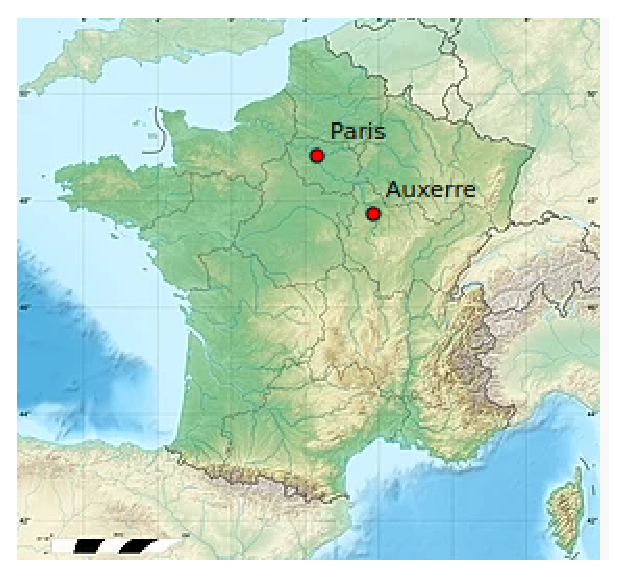
\includegraphics[width=0.65\textwidth]{figs/auxerre-paris}
		\end{center}
		}
		{
			\includegraphics[width=0.45\textwidth]{figs/Fourier2}%\pause
	%	\begin{center}
	%		\includegraphics[width=0.7\textwidth]{figs/tombe-2015}
	%	\end{center}
		}
\end{slide}

\begin{slide}[toc=]{Transformada de Fourier}
 \begin{itemize}
  \item Defini\c c\~oes
     \begin{equation*} X(e^{j\omega})=\sum_{n=-\infty}^{\infty} x[n]e^{-j\omega n}  \end{equation*}
     \begin{equation*} x[n]=\frac{1}{2\pi}\int_{-\pi}^{\pi} X(e^{j\omega})e^{j\omega n} d\omega \end{equation*}
   \item Forma retangular: $X(e^{j\omega}) = X_R(e^{j\omega}) + j X_I(e^{j\omega})$
   \item Forma polar: $X(e^{j\omega}) = |X(e^{j\omega})|e^{j\angle X(e^{j\omega})}$
 \end{itemize}
\end{slide}

\begin{slide}[toc=]{Prova da transformada inversa}
      \begin{align*} x[n]&= \frac{1}{2\pi}\int_{-\pi}^{\pi} X(e^{j\omega})e^{j\omega n} d\omega\\
                       &= \frac{1}{2\pi}\int_{-\pi}^{\pi} \left ( \sum_{m=-\infty}^{\infty} x[m]e^{-j\omega m}\right )e^{j\omega n} d\omega\\
                       & = \sum_{m=-\infty}^{\infty}x[m]\left ( \frac{1}{2\pi} \int_{-\pi}^{\pi} e^{j\omega(n-m)}d\omega \right ) \\   
                       & = \sum_{m=-\infty}^{\infty}x[m] \delta[n-m] = x[n]\end{align*}
\end{slide}

\begin{slide}[toc=]{Exemplos 2}
Calcule a resposta em frequência dos sistemas LI abaixo representados:
\begin{enumerate}
   \item $h_1[n] = a^nu[n], \quad |a|<1$
   \item $h_2[n] = a^{|n|}, \quad |a|<1$
   \item $h_3[n] = \begin{cases} 1,& |n|\leq N_1\\0,&|n|> N_1\end{cases}$
\end{enumerate}
\end{slide}

\begin{note}[toc=]{Exercícios}
Trace os gráficos de magnitude e fase das respostas em frequência dos sistemas de resposta ao impulso $h_1$, $h_2$ e $h_3$ para: 
\begin{enumerate}
   \item $a = 0,9$ ($h_1$ e $h_2$)
   \item $a = -0,9$ ($h_1$ e $h_2$)
   \item $N_1 = 3$ ($h_3$)
   \item $N_1 = 10$  ($h_3$)
\end{enumerate}
Qual o comportamento esperado da transformada de Fourier de $h_3[n]$ quando $N_1\rightarrow 0$ ?
\end{note}

\section[slide=true]{Propriedades da Transformada de Fourier}
\begin{slide}[toc=]{Sinais complexos: simetria e anti-simetria conjugada}
\begin{itemize}
   \item Sequências  simétrica e anti-simétrica conjugada
   \begin{align*}
      x[n] &= x_e[n]+x_o[n]\\
      x_e[n] &= \frac{1}{2} \left \{ x[n] + x^*[-n] \right \} = x_e^*[-n]\\
      x_o[n] &= \frac{1}{2} \left \{ x[n] - x^*[-n] \right \} = -x_o^*[-n]
   \end{align*} 
\end{itemize}
\end{slide}

\begin{slide}[toc=]{Sinais complexos}
\begin{itemize}
   \item Propriedades da transformada de Fourier para sinais complexos
\begin{itemize}
   \item $x^*[n]\stackrel{F}{\leftrightarrow} X^*(e^{-j\omega})$
   \item $x^*[-n]\stackrel{F}{\leftrightarrow} X^*(e^{j\omega})$
   \item $\Re\{x[n]\} \stackrel{F}{\leftrightarrow} X_e(e^{j\omega})$
   \item $j\Im\{x[n]\} \stackrel{F}{\leftrightarrow} X_o(e^{j\omega})$
   \item $x_e[n] \stackrel{F}{\leftrightarrow} X_R(e^{j\omega}) = \Re\{X(e^{j\omega})\}$
   \item $x_o[n] \stackrel{F}{\leftrightarrow} jX_I(e^{j\omega}) = j\Im\{X(e^{j\omega})\}$
\end{itemize}
\end{itemize}
\end{slide}


\begin{slide}[toc=]{Sinais reais}
\begin{itemize}
   \item Propriedade da transformada de Fourier para $x[n]$ real
   \begin{itemize}
      \item $ X(e^{j\omega}) = X^*(e^{-j\omega})$
      \item $ X_R(e^{j\omega}) = X_R(e^{-j\omega})$
      \item $ X_I(e^{j\omega}) = -X_I(e^{-j\omega})$
      \item $ |X(e^{j\omega})| = |X(e^{-j\omega})|$
      \item $ \angle X(e^{j\omega}) = -\angle X(e^{-j\omega})$
      \item $ x_o[n] \stackrel{F}{\leftrightarrow} X_R(e^{j\omega})$
      \item $ x_e[n] \stackrel{F}{\leftrightarrow} jX_I(e^{j\omega})$
   \end{itemize}
\end{itemize}
\end{slide}

\section[slide=true]{Teoremas da transformada de Fourier}
\begin{slide}[toc=]{Teoremas}
\center{
\small{\begin{tabular}{l|l}
\hline
Sequência & Transformada de Fourier \\
\hline
$x[n]$     &   $X(e^{j\omega})$ \\
$y[n]$     &   $Y(e^{j\omega})$\\
\hline
1. $ax[n]+by[n]$ & $aX(e^{j\omega})+bY(e^{j\omega})$\\
2. $x[n-n_d]$ & $e^{-j\omega n_d}X(e^{j\omega})$ \\
3. $e^{j\omega_o n}x[n]$ & $X(e^{j(\omega-\omega_o)})$\\
4. $x[-n]$ & $X(e^{-j\omega})$\\
           & $X^*(e^{j\omega})$ se $x[n]$ for real\\
5. $nx[n]$ & $j\frac{dX(e^{j\omega})}{d\omega}$\\
6. $x[n]*y[n]$ & $X(e^{j\omega})Y(e^{j\omega})$\\
7. $x[n]y[n]$ & $\frac{1}{2\pi}\int_{-\pi}^{\pi} X(e^{j\theta})Y(e^{j(\omega-\theta)})d\theta$\\
\hline
\multicolumn{2}{l}{8. $\sum_{n=-\infty}^{\infty}|x[n]|^2=\frac{1}{2\pi}\int_{-\pi}^{\pi}|X(e^{j\omega})|^2d\omega$}\\
\multicolumn{2}{l}{9. $\sum_{n=-\infty}^{\infty}x[n]y^*[n]=\frac{1}{2\pi}\int_{-\pi}^{\pi}X(e^{j\omega})Y^*(e^{j\omega})d\omega$}\\
\hline
\end{tabular}}}
\end{slide}

\begin{note}{Exercícios}
\begin{enumerate}
   \item Deduza cada uma das propriedades da transformada de Fourier.
   \item Prove cada um dos teoremas da transformada de Fourier. 
\end{enumerate}

\end{note}



\end{document}
